\chapter{Introduction}\label{chapter:introduction}
According to the Lawson criterion, for nuclear fusion to occur, the product of particle density $n$, temperature $T$, and confinement time $\tau$ must be above a critical value.
\begin{align}
	n\,T\,\tau_E \geq 3\times 10^{21}~\frac{\text{keV s}^3}{\text{m}}
\end{align}
The confinement time is generally regarded to be the term that limits progress in development of fusion.
Currently, no experiment has achieved this criterion.

In 1982, a new neutral-beam injection heating system was install in the ASDEX tokamak, which pushed the device into a new realm of operation.
An increased level of energy confinement time was achieved, measured to be a factor of 2 or more than what was expected.
This state of operation was coined the high-confinement (H--) mode, and is now considered necessary for the future of nuclear fusion as an energy source \cite{arnoux_how_2009, wagner_development_1984}.
With this new level of energy confinement, the community got one step closer to economic fusion power plants.
The details of this transition, however, are not fully understood.

\section{Characteristics of L-- and H--Mode}\label{sec:characteristics}
Transport of particles and energy in tokamaks has been discovered to be significantly dominated by anomalous (turbulent) transport, which is generally assumed to be generated by turbulence, which are driven by micro-instabilities.
Low-confinement mode, referred to as L--mode, is dominated by this transport at the edge.
The formation of H--mode is due to the suppression of this turbulent transport at the edge of the plasma.
This mode is therefore categorized as having a transport barrier.
The plasma edge is defined to be the thin boundary layer of the plasma just inside the last-closed flux surface.

\begin{figure}[tb] % L--H-modes compare
\begin{minipage}{0.49\linewidth}
	\centering
	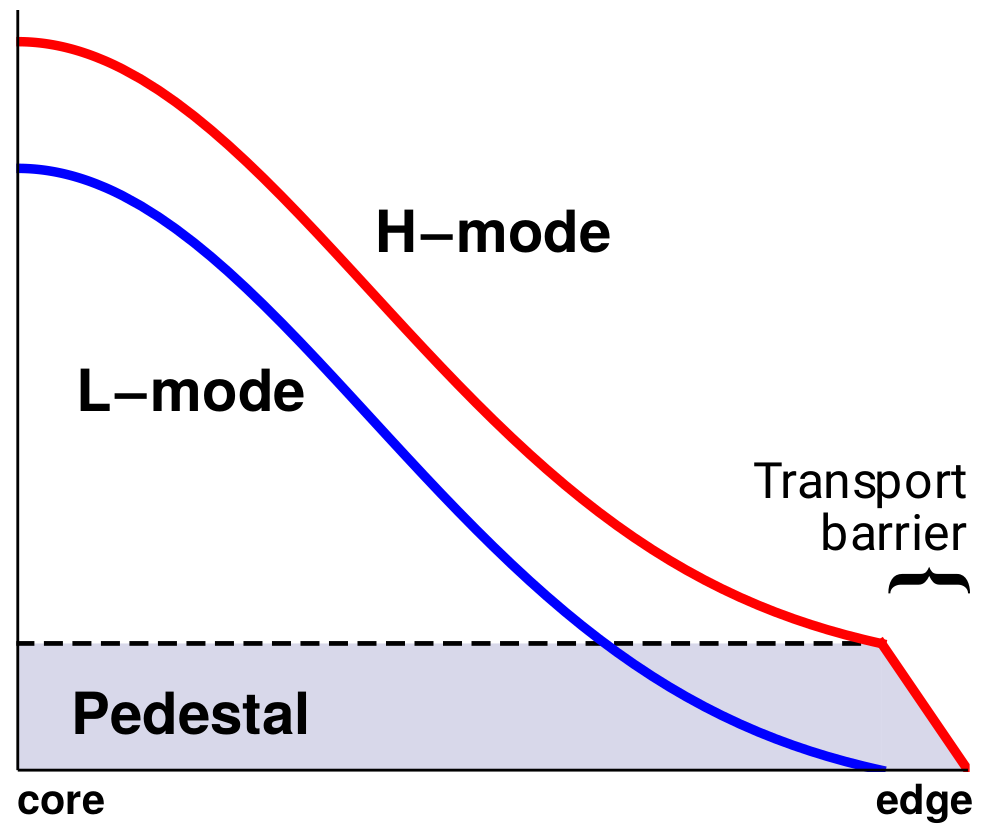
\includegraphics[width=0.8\textwidth]{../Graphics/L-mode_H-mode_compare.png}
\end{minipage}
\hfill
\begin{minipage}{0.49\linewidth}
	\caption{A comparison of the radial pressure profiles of L--mode and H--mode.
	The profile of H--mode can be thought of as on a ``pedestal,'' in which the pressure profile is increase in the core.
	This is due to the transport barrier that is formed at the edge \cite{weymiens_bifurcation_2014}.}
	\label{fig:L-mode_H-mode_compare}
\end{minipage}
\end{figure}

One of the properties of H--mode is its significantly-raised pressure profile compared to that of L--mode, and is said to sit on a ``pedestal.''
Accordingly, there is a steep gradient in the pressure at the edge of the plasma, shown and compared to L--mode in Figure~\ref{fig:L-mode_H-mode_compare} \cite{weymiens_bifurcation_2014}.
This allows for an increased temperature in the core.

In addition, hysteresis is present between the modes, in which the threshold power for the transition between the two modes is based on the current mode.
This is covered in-depth in Section~\ref{ssec:hysteresis}.

\section{The L--H Transition}\label{sec:the_transition}
The key feature that determines a divertor tokamak's operational mode is the amount of external heating power.
Limiter tokamaks (without biasing) are relegated to stay in L--mode, as H--mode is an exclusive operating mode of tokamaks with divertors.
The transition has been observed to occur in one of three general manners: sharp, smooth, and oscillatory.
\todo{\color{red}WHERE TO MOVE THIS small section!?}

\section{Research Questions}\label{sec:research_questions}
Although there have been compilations of different theories describing the transition, there is yet to be a conclusive, comprehensive one \cite{connor_review_2000}.
There is substantial evidence, both theoretically and experimentally, that a radial electric field is an essential piece in the forming and enforcing of H--mode.
Many of the effects in generating and suppressing the field show up as additive terms in an equation for a radial displacement current.
Because many of these fluxes scale differently, simple scaling laws for H--mode could contrast for regimes where different effects dominate.
It is therefore important to evaluate which terms dominate in their respective regimes before inquiring about global scalings.
The overall problem is thus stated simply: \textbf{Which electric field-generating terms are dominant in concrete experimental tokamak conditions?}
This is in an effort to determine which measurable and controllable values can predict H--mode.

The first consideration is to decide \textbf{which terms should be considered for investigation}, as not all nonambipolar fluxes will significantly contribute to the transition.
For example, the nonambipolar flux due to magnetic ripple loss highly depends on collisionality, in which lower collisionality results in a low flux \cite{stringer_effect_1972}.
Since a relatively ideal operation (temperature on the order of 100 eV at the edge) will be investigated, this flux can be neglected.

\textbf{Identifying what optimal form and relative strengths of each flux and subsequently implementing them} appropriately is the crucial next step.
Because the model is highly nonlinear, it is sensitive to the forms and relative strengths.
The calculation is done with a finite volume method solver, in which the results requires verification with the literature.

The main input heating power regime previously investigate was strictly limited to near the H--L transition \cite{staps_backstepping_2017}.
Performing a scan of input heating power significantly above the lower threshold could show a difference in behavior of the fluxes and resulting field.
Therefore, \textbf{what is the variation in dominance of each field-generating term across increasing input power}, including those inside and outside the regime with non-unique operational modes?

\todo{\color{red}OUTLINE of thesis}.

